\documentclass{article}
\usepackage{float} 
\usepackage{graphicx}
\usepackage{mdframed}
\usepackage{tikz}

\title{Documentazione progetto Ingegneria del Software \\  
        \large{Software per la gestione di pazienti diabetici} }

\author{Toffali Tommaso - VR 500800}
        
\date{August 2026}

\begin{document}

\maketitle

\newpage

\tableofcontents

\newpage
\section{Requisiti e Use Case}

\subsection{Requisiti}
Il software sviluppato è un sistema di telemedicina di un servizio clinico per la gestione di pazienti diabetici. Il sistema permette l'interazione di due attori principali: il diabetologo e il paziente. Questi creano un nuovo utente che, dopo essere stato verificato da un admin, finiscono di creare il loro profilo con i dati relativi al ruolo scelto. \\
Una volta autenticato ogni utente verrà reindirizzato alla propria pagina home, nella quale visualizzerà le azioni e informazioni relative al proprio ruolo. Di seguito è presente un diagramma che rappresenta i casi d'uso per ogni utente dopo la corretta autenticazione.

\begin{figure}[H]
    \centering
    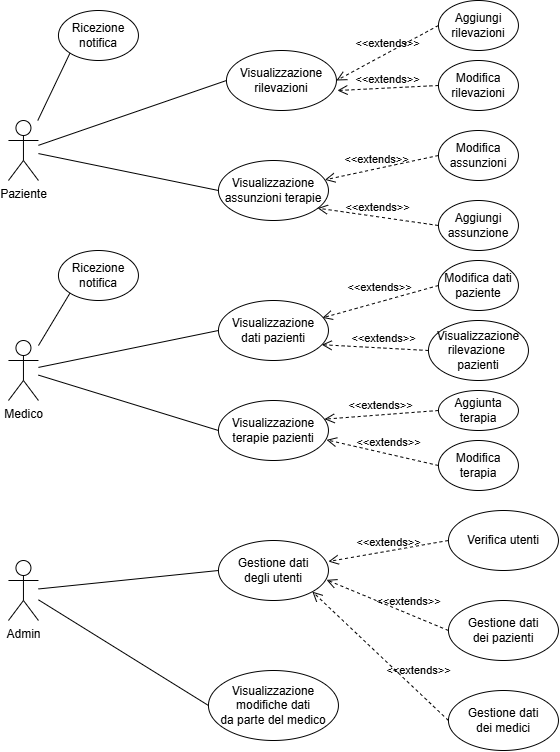
\includegraphics[width=0.6\linewidth]{images/UseCases.png}
    \caption{Casi d'uso per ruolo}
    \label{use cases}
\end{figure}


%% Per il disegno degli use cases controllare il pacchetto tikz-uml, qui sotto abbiamo una prova
\subsection{Casi d'uso paziente}
Dopo che il paziente si è autenticato ed entra nella sua pagina home dove visualizza tutte le azioni a lui disponibili.

\subsubsection{Inserimento o modifica rilevazioni}
Una delle pagine disponibili per il paziente è quella di visualizzazione delle rilevazioni passate che sono state effettuate, con relativa possibilità di modifica di queste, e la possibilità di registrare i dati di una nuova rilevazione.
\begin{mdframed}
    \textbf{Attore:} Paziente \\
    \textbf{Precondizioni:} il paziente deve essersi autenticato correttamente \\
    \textbf{Passi}:
    \begin{enumerate}
        \item Il paziente dalla home page accede alla pagina di visualizzazione e modifica delle rilevazioni.
        \item Il paziente può:
        \begin{itemize}
            \item inserire i dati per una nuova rilevazione: livelli di glicemia, se è stata effettuata prima o dopo un pasto, data e ora.
            \item modificare i dati di una rilevazione passata, tranne la data e ora.
            \item Può inserire eventuali sintomi.
        \end{itemize}
        \item Il paziente conferma l'inserimento della rilevazione.
    \end{enumerate}
    \textbf{Postcondizioni:} La rilevazione viene salvata/aggiornata e se i livelli di glicemia sono al di fuori del normale viene inviata una notifica al medico di riferimento del paziente.
\end{mdframed}

\begin{figure}[H]
    \centering
    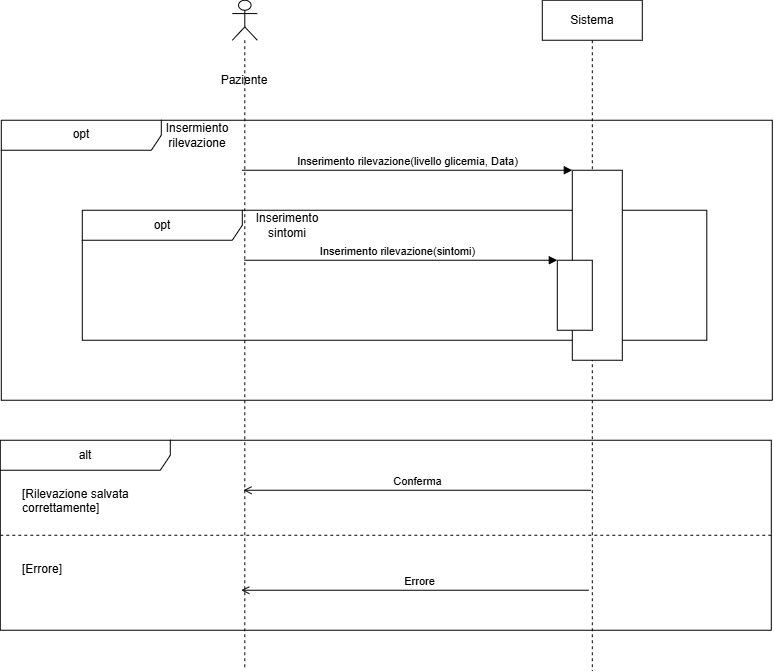
\includegraphics[width=1\linewidth]{images/SeqDiaRilevazione.png}
    \caption{Sequence diagram per inserimento rilevazione paziente}
    \label{Sequence diagram rilevazione}
\end{figure}

\subsubsection{Inserimento assunzione farmaco}
Un'altra pagina disponibile per il paziente riguarda la visualizzazione delle terapie che gli sono state prescritte dal medico, con relativa possibilità di aggiungere una nuova assunzione di un farmaco tra quelli che ha presenti nelle terapie.
\begin{mdframed}
    \textbf{Attore:} Paziente \\
    \textbf{Precondizioni:} il paziente deve essersi autenticato correttamente \\
    \textbf{Passi}:
    \begin{enumerate}
        \item Il paziente dalla home page accede alla pagina di visualizzazione delle terapie e assunzioni di farmaci.
        \item Il paziente preme il bottone per inserimento di una nuova assunzione:
        \begin{itemize}
            \item Inserisce la medicina assunta, la quantità presa, la data e ora.
        \end{itemize}
        \item Il paziente conferma l'inserimento dell'assunzione.
    \end{enumerate}
    \textbf{Postcondizioni:} L'assunzione del farmaco viene salvata nel sistema, questo controlla che l'assunzione sia regolare con la terapie prescritta dal medico e in caso negativo notifica il medico di riferimento.
\end{mdframed}


\subsection{Casi d'uso medico}
Dopo che il medico si è autenticato ed entra nella sua pagina home dove visualizza tutte le azioni a lui disponibili.
\subsubsection{Visualizzazione dei dati del paziente}
\begin{mdframed}
    \textbf{Attore:} Medico \\
    \textbf{Precondizioni:} Il medico deve essere autenticato correttamente \\
    \textbf{Passi:}
    \begin{enumerate}
        \item Il medico dalla sua pagina home accede alla pagina di visualizzazione dati dei pazienti.
        \item Il medico visualizza una lista dei suoi pazienti con i suoi dati principali.
    \end{enumerate}
    \textbf{Postcondizioni:}nessuna
\end{mdframed}

\subsubsection{Modifica dei dati del paziente}
\begin{mdframed}
    \textbf{Attore:} Medico \\
    \textbf{Precondizioni:} Il medico deve essere autenticato correttamente \\
    \textbf{Passi:}
    \begin{enumerate}
        \item Il medico dalla sua pagina home accede alla pagina di visualizzazione dati dei pazienti.
        \item Il medico visualizza una lista dei suoi pazienti con i suoi dati principali.
        \item Il medico seleziona l'azione di modifica che si trova a fianco di ogni riga di un paziente.
        \item Il medico può modificare i dati relativi a fattori di rischio del paziente.
        \item Il medico conferma le modifiche dei dati del paziente.
    \end{enumerate}
    \textbf{Postcondizioni:} Il sistema modifica i dati del paziente e viene salvata nella lista delle tracce.
\end{mdframed}

\subsubsection{Modifica o aggiunta di terapie}
\begin{mdframed}
    \textbf{Attore:} Medico \\
    \textbf{Precondizioni:} Il medico deve essere autenticato correttamente \\
    \textbf{Passi:}
    \begin{enumerate}
        \item Il medico dalla sua pagina home accede alla pagina di visualizzazione delle terapie.
        \item Il medico visualizza una lista delle terapie che sono collegate ai suoi pazienti.
        \item Il medico può:
        \begin{itemize}
            \item modificare una terapia già assegnata.
            \item aggiungere una nuova terapia ad un paziente.
        \end{itemize}
        \item Il medico conferma le modifiche che ha effettuato.
    \end{enumerate}
    \textbf{Postcondizioni:} Il sistema modifica i dati della terapia che è stata aggiunta/modificata.
\end{mdframed}

\subsection{Casi d'uso admin}
L'amministratore del sistema gestisce gli utenti del sistema, si occupa di modificare/cancellare account di pazienti e medici. La registrazione viene effettuata tramite un form dove viene specificato il ruolo, prima che un utente possa utilizzare le funzioni relative al suo ruolo nel sistema l'amministratore deve autorizzare la richiesta di creazione dell'account da parte dell'utente

\subsubsection{Gestione degli utenti}
\begin{mdframed}
    \textbf{Attore:} Admin \\
    \textbf{Precondizioni:} L'admin deve essere autenticato correttamente \\
    \textbf{Passi:}
    \begin{enumerate}
        \item L'admin dalla sua pagina home accede alla pagina di gestione degli utenti
        \item L'admin visualizza la lista degli utenti
        \item L'admin può:
        \begin{itemize}
            \item Modificare un utente
            \item Eliminare un utente
        \end{itemize}
    \end{enumerate}
    \textbf{Postcondizione:} L'utente è stato modificato o eliminato.
\end{mdframed}

\subsubsection{Gestione delle richieste di registrazione}
\begin{mdframed}
    \textbf{Attore:} Admin \\
    \textbf{Precondizioni:} L'admin deve essere autenticato correttamente \\
    \textbf{Passi:}
    \begin{enumerate}
        \item L'admin dalla sua pagina home accede alla pagina di gestione degli utenti
        \item L'admin visualizza la lista degli utenti
        \item L'admin può:
        \begin{itemize}
            \item Accettare la richiesta di registrazione di un utente
            \item Rifiutare la richiesta di registrazione di un utente
        \end{itemize}
    \end{enumerate}
    \textbf{Postcondizione:} Se accettata l'utente viene verificato e può procedere con il completamento dei dati, altrimenti niente.
\end{mdframed}

\subsubsection{Visualizzazione delle modifiche dei medici}
Il sistema tiene traccia delle modifiche che i medici effettuano sui pazienti

\begin{mdframed}
    \textbf{Attore:} Admin \\
    \textbf{Precondizioni:} L'admin deve essere autenticato correttamente \\
    \textbf{Passi:}
    \begin{enumerate}
        \item L'admin dalla sua pagina home accede alla pagina di visualizzazione delle modifiche da parte dei medici
        \item L'admin visualizza la lista delle modifiche effettuate
    \end{enumerate}
    \textbf{Postcondizione:} Nessuna
\end{mdframed}


\subsection{Activity diagram}

\subsubsection{Registrazione di un utente}
Solamente pazienti e medici posso registrarsi al sistema, la loro registrazione consente nella creazione di un utente con il proprio ruolo, una volta verificato dall'admin questo può terminare la registrazione completando i dati per il ruolo che ha scelto.

\begin{figure}[H]
    \centering
    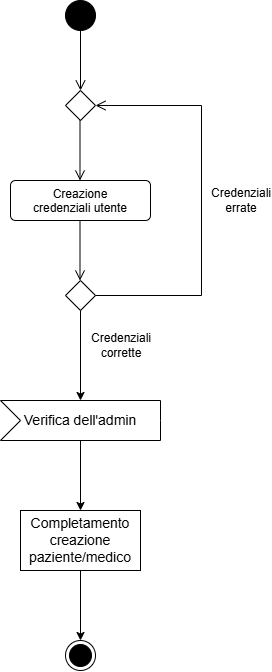
\includegraphics[width=0.5\linewidth]{images/RegistrazioneUtente.png}
    \caption{Registrazione da parte di un utente}
    \label{RegistrazioneUtente}
\end{figure}

\subsubsection{Attività del paziente}
Di seguito è presente un activity diagram per un paziente in seguito alla corretta autenticazione al sistema.

\begin{figure}[H]
    \centering
    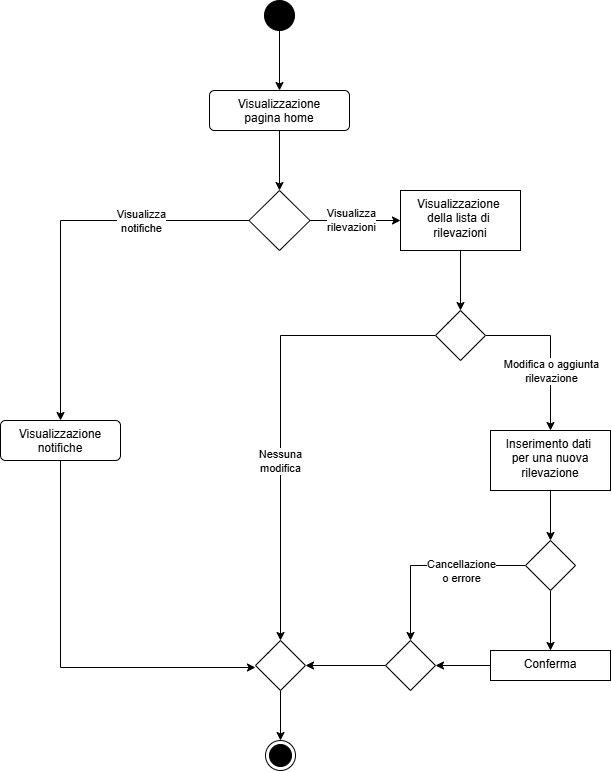
\includegraphics[width=0.8\linewidth]{images/ActivityPaziente.png}
    \caption{Activity diagram di un Paziente}
    \label{ActivityPaziente}
\end{figure}

\subsubsection{Attività del medico}
Di seguito è presente un activity diagram per un medico in seguito alla corretta autenticazione al sistema.

\subsubsection{Attività dell'amministratore}
Di seguito è presente un activity diagram per un admin in seguito alla corretta autenticazione al sistema.



\newpage
\section{Sviluppo}

\subsection{Processo di sviluppo}
Il lavoro svolto per la realizzazione del progetto e' stato 
Il team è composto da due sviluppatori che hanno lavorato in parallelo sulle diverse funzionalità fornite dal sistema. Ogni qualvolta che venivano decise le funzionalità da implementare veninavano divise in base al ruolo su cui venivano svolte, per ogni task svolta e testata questa veniva passata anche all'altro membro che la testava a sua volta e ne dava dei riscontri.\\
Per la gestione del codice è stato utilizzato \textit{git} come sistema di versionamento
\subsection{Progettazione e pattern utilizzati}
Il progetto segue un'architettura del tipo \textit{Client-Server} ispirata al pattern \textit{Model-View-Controller (MVC)}. Il sistema è diviso in due parti:
\begin{itemize}
    \item \textbf{Client:} si occupa dell'interfaccia ed è ciò con cui l'utente interagisce. L'implementazione è stata possibile tramite un framework per applicazioni web, \textit{Angular Material}, che tramite richieste HTTP comunica al server per ricevere e modificare dati.
    \item \textbf{Server:} realizzato con \textit{Spring boot}, espone delle API che il Cliente invoca con le richieste HTTP per lo scambio dei dati, gestisce sia la logica di business (Model) che il controllo delle richieste (Controller).
    \begin{itemize}
        \item \textbf{Model:} rappresenta le entità principali del sistema, come ad esempio \textit{Pazienti}, \textit{Medici}, \textit{Rilevazioni}, \textit{Notifiche} e  il \textit{Change log}.
        \item \textbf{Controller:} gestisce le richieste che provengono dal client e le invia al Model per la gestione dei dati. 
    \end{itemize}
\end{itemize}
Questa scelta di architettura permette di separare le responsabilità tra le due parti del sistema, rendendo più semplice la manutenzione e l'evoluzione del software. Inoltre, l'utilizzo del pattern MVC consente di avere una chiara distinzione tra la logica di business e la presentazione dei dati, facilitando lo sviluppo e il testing delle singole componenti.
\subsection{Implementazione e design pattern utilizzati}



\newpage
\section{Test e validazione}

\subsection{Revisione}
\subsection{Test}
\subsection{Test manuali}
\subsection{Test da parte di utenti}


\end{document}
